\documentclass[letterpaper,12pt]{article}
\usepackage[utf8]{inputenc}

\usepackage[T1]{fontenc}
\usepackage{tgtermes} %%%font

\usepackage{geometry}
\usepackage{amsmath}
\usepackage{float}
\usepackage{graphicx}
\usepackage{subcaption}
\usepackage{amssymb}
\usepackage{adjustbox}
\usepackage{wrapfig} %%imagen envuelta por un texto
\usepackage{xcolor}
\usepackage{fancyhdr}
\usepackage{tabularx} %%TABLAS OH YEAH

\title {\textbf{Evolución de la Administración}}
\author{Lara Xocuis Martha Denisse}
\date{12 de septiembre de 2023}
\geometry{top=2cm, bottom=2cm, left=2cm, right= 2cm} %%margen
\graphicspath{{images/}}
\parindent=0pt

\begin{document}
\maketitle

%%%%%%%%%%%%%%%%%%%%%%%%%%%%%%%%%%%%%%%%%%%%%%%%%%%%%%%%%%%%%%%%%%%%%%%%%%%%
\begin{sloppypar}
\begin{enumerate}
    \item Escuela clásica/tradicional : La evolución histórica de la gestión empresarial, tiene un desenvolvimiento de ideas a nivel culturales en oriente y occidente,alcanzado el desarrollo del hombre en cada uno de los sistemas sociales por lo que ha pasado, (Fernandez, 2005), ya que ha evolucionado la toma decisiones analizando sus cuatros funciones claves para el desarrollo de mando a nivel empresarial, como lo son; planificar, organizar, dirigir y controlar, por consiguiente una gestión y persona dinámica en el mundo empresarial en el desenvolvimiento de un entorno y mercado competitivo y productivo a una escala mundial. Hay una gran diversidad de teorías, enfoques y pensadores del tema que estamos tratando, a continuación describimos cada de los elementos anteriormente mencionados.

    La empresas, en este terreno tanto por lo que se refiere a la prácticas diversas llevadas a cabo en las empresas como a teorías sobre el comportamiento administrativos de las personas, evolución del conocimientos, enseñanza de la materia y diversos aspectos relaciónados(Castilla, 2005). La realidad de nuestro entorno más ideal y complejo, en todo descubriremos y desarrollaremos en unos ambientes únicos en el mundo de los negocios, esta dimensión hacen pensar que las actividades la haremos de una diferente, en la operación de mercados geográficos cada día, diferente lo que fue ayer, en el hoy y un mañana cada variado y dinámico, por consiguiente debemos tener muy claro las bases teóricos para desenvolvimiento de nuestras empresas, con gran variedad, es por la dirección de empresa está experimentado, la ampliación y diversificación de diferentes enfoques en el desarrollo de nuevos temáticas para la consecución de nuevos logros y estándares en los fenómenos organizativos… con la consecución de nuevas estrategias y la utilización de recursos como son; humanos, producción, marketing, operaciones, economía, finanzas y contabilidad (Berreiro Fernández, Diez de Castro, Barreiro Fernández, Ruzo Sanmartín, y Lozada Pérez, 2003).


    \item Escuela empírica: La escuela  empírica  de la  administración es  un  modelo  que  analiza  la  gestión  a través de la experiencia. Como un estudio de la práctica, crea una generalización, pero habitualmente como un medio para enseñar la experiencia al profesional o al estudiante. Es la escuela administrativa que busca conseguir los resultados deseados a través de  la  aplicación  de  un  esquema  adquirido  de  ejemplos  que  ya  han  sido comprobados y su éxito se puede confirmar.
    \item Escuela comportamental: Diversos autores y académicos, muchos de ellos especializados en administración de empresas, mercadotecnia y liderazgo corporativo, se han preocupado por darle un marco teórico a este concepto.

    Para Stephen Robbins, un autor estadounidense de libros de gestión empresarial, el comportamiento organizacional “es un campo de estudio que investiga el impacto de los individuos, grupos y estructuras sobre el comportamiento dentro de las organizaciones”.
    
    Mientras tanto, los académicos Keith David y John Newstrom, también estadounidenses, lo definen como “el estudio y la aplicación de conocimientos relativos a la manera en que las personas actúan dentro de las organizaciones”.
    
    Como ves, el comportamiento organizacional es mucho más que la interacción entre trabajadores, grupos y estructuras de una empresa, pues se ocupa del análisis de cómo estas variables influencian el desarrollo del talento humano y el funcionamiento en general.
    
    Este concepto y todos su sus elementos se aplican y adoptan como filosofía con un fin mayor: promover el desarrollo humano dentro de las empresas y organizaciones.
    El comportamiento organizacional cuenta con diferentes teorías centradas en campo de estudio específicos, lo que permite que este concepto sea amplio y completo.

    Específicamente, está integrado por estas 5 teorías:

    Teoría clásica
    Se enfoca en la necesidad de encontrar elementos para administrar organizaciones complejas.

    Teoría de la administración científica
    Busca la perfección de las técnicas de trabajo y la creación de parámetros capaces de medir la eficiencia.

    Teoría de las relaciones humanas
    Prioriza a los individuos sobre los otros elementos de las organizaciones y sugiere estrategias para aumentar la satisfacción de cada uno.

    Teoría de los sistemas
    Es una filosofía administrativa basada en sistemas, es decir, en conjuntos de elementos que se relacionan entre sí para constituir un “todo organizado”, que brinda mejores resultados que la suma de partes.

    Teoría de contingencia
    Enfatiza que no hay nada absoluto en las empresas e instituciones y que, en cambio, todo es relativo.

    \item Escuela teoríca de decisión:  
    Entre  los  promotores  de  la  escuela  de  la  teoría  de  las  decisiones  están  Herbert Simon, March y Simon, quienes proponen la aceptación de la metodología de la toma  de  decisiones  en  la  administración.  Así  como  también  Von  Newman, Bowman  y  Hutchinson,  quienes  más  han  contribuido  a  este  enfoque.

    Herbert  a. Simon  utilizó esta  teoría  para  explicar el  comportamiento del  ser  humano en las organizaciones, partiendo de la base de que todas las personas que trabajan en la  empresa  toman  decisiones  y  esto  es  importante.

    Esta escuela considera que la tarea más importante de los administradores es la toma de las decisiones, ya que “todo el proceso administrativo puede explicarse en  términos  de  tomas  de  decisiones”;  o  lo  que  es  lo  mismo,  tomar  decisiones representa el verdadero trabajo del administrador y se define como la selección más  conveniente  de  un  curso  de  acción  entre  dos  o  más  cursos  de  selección. alternos;  es  decir,  escoger  una  alternativa  entre  las  disponibles  para  resolver  la situación, problema, dificultad o conflicto que se esté presentando. En la toma de decisiones  importa la  elección  de  un camino  a  seguir, por lo que en un estadio anterior  deben  evaluarse  alternativas  de  acción. 

    Su principal énfasis lo hace en la decisión Racional o sea el proceso decisorio se basa en hechos. (Existe también el intuitivo que se basa en valores). Esto significa que el administrador debe utilizar el modelo racional, aunque en el momento de decidir  surgen  sus  valores  que  van  implícitos  en  la  decisión.
    \newpage
    \item Escuela gestión de sistemas: Esta teoría estudia a las organizaciones como sistemas sociales que se encuentran en constante relación con otros sistemas que afectan y son afectados por los otros sistemas. George Braziller define a los sistemas como: Un todo organizado, compuesto por dos o más partes, componentes o subsistemas, y delineado por los límites identificables de su ambiente o supra sistema. 

    Los sistemas se clasifican en base a diversos criterios:
    
    Por su composición material y objetiva: abstracto y concreto.
    
    Por la movilidad interna: estático, dinámico, homeostáticos y probabilísticos.
    
    Por el grado de interacción entre otros sistemas: abiertos y cerrados.
    
    Por el grado de dependencia: independientes y dependientes.
    
    Por capacidad de respuesta: pasivos, activos y reactivos. 
    
    Elementos de los sistemas: básicamente cada sistema cuenta con cuatro elementos, insumos o influjos, procesos, producto y retroalimentación

    \begin{figure}[H]
        \centering 
        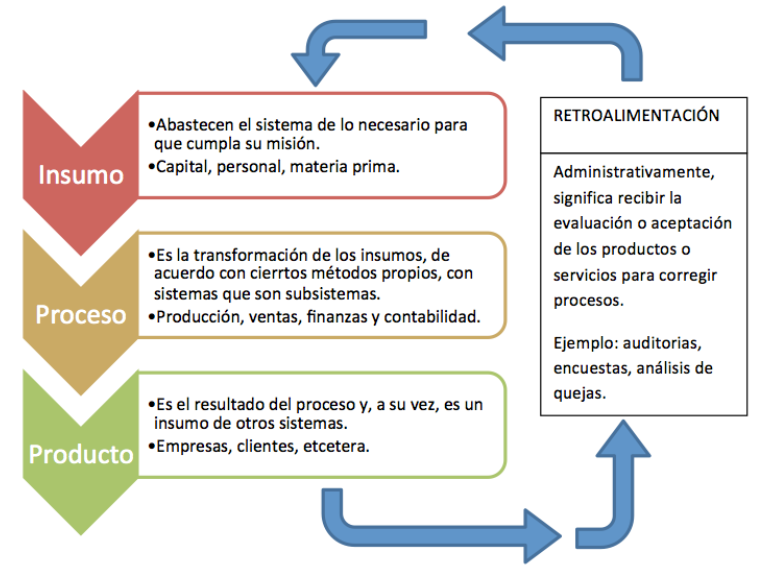
\includegraphics[width=0.6\textwidth]{images/sis.png}
    \end{figure}
    \item Gestión del conocimiento: La gestión del conocimiento –a nivel empresarial– se define como un conjunto de actividades y procesos con el objetivo de facilitar la creación, organización e intercambio de información entre los clientes y funcionarios de la compañía.

    El objetivo principal de la gestión del conocimiento es mejorar la experiencia de los consumidores y optimizar los resultados en productividad e innovación de la empresa.

    Para lograrlo, la gestión del conocimiento busca:
    
    la creación y difusión de información, tanto en la organización como entre ella y sus clientes;
    entender cómo hacer que las compañías sean más competitivas y adaptables;
    aplicar procesos y mecanismos de gestión para agilizar el aprendizaje.
    El 51\% de los clientes prefiere soporte técnico a través de una base de conocimientos. Un sistema de gestión de la información te provee de herramientas para hacer que el conocimiento se vuelva mucho más accesible y que el servicio de atención se agilice gracias al autoservicio.

    \item Maquila: Maquila es un término que se usa en el contexto de la administración, de la organización de la empresa, negocios y gestión. En concreto, suele ser utilizado para hablar de aquellos inputs o tecnologías que se adquieren importándose y empleándose una mano de obra local, destinada a producir productos para su posterior exportación.

    En concreto, la maquila permite a las empresas poder producir los productos y servicios que ellas desean a un coste de la mano de obra del país más económico. Tampoco tienen en cuenta los costes de los aranceles vigentes en dicho país.
    
    El país receptor de la maquila se ve beneficiado al entrar nuevas materias primas y mano de obra a su país, así como de la generación de empleo, por lo que la economía regional será impulsada (a menos que la mano de obra sea subcontratada).
    
    En algunos países como Paraguay o México, la producción mediante maquilas puede permitir la importación temporal con suspensión de impuestos sobre estas materias primas que serán necesarias para la fabricación de los productos. Esto puede ser muy ventajoso para las empresas, pues pueden ahorrarse una gran cantidad, y consecuentemente obtener más beneficios.

    \item Justo a Tiempo: Hay varios principios y filosofías que guían la producción industrial, desde la más antigua y tradicional hasta la más moderna, tecnológica y ultrarrápida. En este conjunto de ideas, justo a tiempo (just in time), o en el momento adecuado en traducción, es una de las principales en el modelo personalizado.

    Esto se debe a que, debido a otros principios, como la economía y la producción efectiva, los productos personalizados se adaptan mejor a un modelo de producción bajo demanda, evitando así el desperdicio innecesario y el retrabajo.
    
    Gracias al éxito de la metodología en la producción a medida, varias de sus características se han adaptado a otros modelos de producción distintos a los personalizados.

    usto a tempo o just in time, que significa «momento adecuado» o «en el momento adecuado», es una filosofía y un sistema que tiene como objetivo producir una cantidad exacta de un producto determinado, a medida que surge la demanda.

Es un modelo centrado en el sistema de producción que determina que nada debe ser producido, transportado o comprado antes del momento adecuado, sin necesidad de acumulación de stock.

Esto genera un impacto significativo en la cadena de producción al desplazar los materiales y materias primas en la cantidad exacta para la producción de una demanda específica de producto en un período de tiempo determinado (generalmente el tiempo de producción establecido en la venta).

Cuando se aplica a la organización, justo a tiempo es muy importante para ayudar a reducir los inventarios y costos derivados del proceso, siendo ampliamente utilizado por las empresas, especialmente de vehículos automotrices – como es el caso de Toyota.

usto a tempo o just in time, que significa «momento adecuado» o «en el momento adecuado», es una filosofía y un sistema que tiene como objetivo producir una cantidad exacta de un producto determinado, a medida que surge la demanda.

Es un modelo centrado en el sistema de producción que determina que nada debe ser producido, transportado o comprado antes del momento adecuado, sin necesidad de acumulación de stock.

Esto genera un impacto significativo en la cadena de producción al desplazar los materiales y materias primas en la cantidad exacta para la producción de una demanda específica de producto en un período de tiempo determinado (generalmente el tiempo de producción establecido en la venta).

Cuando se aplica a la organización, justo a tiempo es muy importante para ayudar a reducir los inventarios y costos derivados del proceso, siendo ampliamente utilizado por las empresas, especialmente de vehículos automotrices – como es el caso de Toyota.
\begin{itemize}
    \item Producción sin stock 
    \item Asignación de recursos bajo demanda 
    \item Producción de acuerdo a la necesidad productiva 
    \item Eliminación de residuos 
    \item Fabricación de flujo continuo 
    \item Esfuerzo continuo en la resolución de problemas
\end{itemize}

    \item Clústers industriales: Un clúster es una especie de concentración de empresas en una zona geográfica determinada o la concentración de diferentes organizaciones relacionadas con una materia concreta y que están presentes en un Estado o región. La razón de ser de estos clústeres es que consiguen aumentar la productividad de las empresas.

    La definición de clúster empresarial, por tanto, no es más que la concentración geográfica de proveedores especializados, compañías interconectadas, socios de industrias, proveedores de servicios e instituciones relacionadas que operan en un campo específico y al que están vinculadas de diferente forma.

    \item GLobalización: La globalización de la administración es una realidad de la vida diaria. Todos los días, los periódicos están
    llenos de noticias que nos recuerdan que las organizaciones han adoptado un enfoque global. Los noticieros
    hablan, con frecuencia de asuntos como las balanzas comerciales internacionales y las fluctuaciones de las
    monedas. No es raro leer acerca de empresas japonesas que están avanzando en los mercados de Estados
    Unidos ni de empresas estadounidenses que están progresando en los mercados de Japón. Se nos informa
    de administradores de los países que estaban tras la “cortina de hierro” que ahora se preparan en Europa
    Occidental o Estados Unidos y de empresas estadounidenses y británicas que se unen para ofrecer nuevos
    servicios de telecomunicaciones y viajes en avión. Hoy, ningún gerente se puede dar el lujo de suponer que
    su organización esta aislada de todas estas actividades mundiales. Los clientes de los chips de Sumitomo,
    como Hewlett – Packard, son testigos de esta afirmación.
    Hoy, no es nada raro encontrar una organización global, con oficina matriz en Estados Unidos, que cuente
    con operaciones fabriles en, por decir algo, Estados Unidos, Alemania y Singapur; que venda sus productos
    en docenas de países llamados “Cuatro Tigres” Hong Kong, Singapur, Corea del Sur y Taiwán.
    Las grandes organizaciones no son las únicas que han optado por la vía global, también es cada vez mayor
    la cantidad de pequeñas empresas que lo hacen. La Globalización es el Reconocimiento por parte de las
    organizaciones, de que las organizaciones deben tener un enfoque global y no un enfoque local. también
    puede esta ser definida de muchas maneras, dependiendo de que nivel se desee analizar, se puede hablar de
    la globalización del mundo entero, de un país, industrias especificas, empresas, hasta de un modelo
    económico y político.
    A escala mundial, la globalización se refiere a la creciente interdependencia entre los países, tal como se
    refleja en los flujos internacionales de bienes, servicios, capitales y conocimientos.
    A escala nacional, se refiere a la magnitud de las relaciones entre la economía de una nación y el resto del
    país.
    Es un proceso de crecimiento internacional o mundial del capital financiero, industrial, comercial, recursos,
    humano, político y de cualquier tipo de actividad intercambiable entre países

    \item Alianzas estratégicas: Las alianzas estratégicas son acuerdos entre dos o más empresas para alcanzar un objetivo común. Son un medio eficaz de obtener recursos rápidamente para entrar en un nuevo mercado, desarrollar nuevos productos e intercambiar servicios o tecnologías que mejoren y mantengan la ventaja competitiva. 

    Estas ayudan a equilibrar las transacciones de mercado ajustándose a los cambios constantes del entorno (Carvajal et al., 2021). Son fundamentales para cualquier negocio o empresa, ya que les permite aprovechar sinergias en proyectos complejos. De esta manera, uniendo sus fuerzas les resulta menos costoso introducirse en un nuevo mercado. 
    
    No se trata de una red de contactos (por lo que es importante saber qué es el networking, una práctica para construir conexiones), sino de uniones formales cuyo propósito es la competitividad y el fortalecimiento de las empresas (Encolombia.com, s.f.).

    \item Organizaciones virtuales:  Las organizaciones virtuales son formas organizativas nuevas, que resultan de: primero,
    reemplazar las interacciones cara a cara con interacciones remotas, soportadas por
    comunicaciones electrónicas y segundo, proveer acceso en tiempo real a toda la información
    de la empresa para todos los trabajadores. La Organización Virtual o también llamada la Organización en Red, se basa en la contratación de empresas independientes para realizar aquellas actividades en las cuales son mejores asociándose en una red, que actúa como una sola empresa.

    Las organizaciones virtuales tienen como objetivo principal la flexibilidad, y son muy parecidas a las organizaciones en trébol y en red. Son organizaciones orientadas al mercado, que se configuran como un conjunto de cadenas de valor relacionadas entre proveedores, clientes, competidores, otras organizaciones y la propia empresa. 

    \item Franquicias: La franquicia es un sistema de comercio asociado entre empresas financieras y jurídicamente independientes, pero ligadas por un contrato en virtud del cual, una de ellas (la franquiciadora) concede a la otra u otras (franquiciados), a cambio de unas contraprestaciones económicas, el derecho a explotar una marca y/o una fórmula comercial materializada en unos signos distintivos, asegurándole la ayuda técnica y los servicios regulares necesarios destinados a facilitar dicha explotación. Es importante tener claro qué es una franquicia y cómo funciona, y en las próximas líneas te lo vamos a contar.
    
    \item e-commerce:  El comercio electrónico empresarial es la compra y venta de productos a grandes empresas u organizaciones. Si una gran empresa vende muchos tipos de productos diferentes o tiene varias líneas de marca y pasa a vender en Internet, entonces participa en el comercio electrónico empresarial.

    \item Teoría de restricciones: En el ámbito de la gestión de proyectos, la teoría de las restricciones (TOC o theory of constraints) es una metodología de resolución de problemas que te ayuda a identificar los obstáculos más importantes o el factor limitante que se interpone en el camino de los objetivos y metas de tu proyecto. Por ejemplo, imagina que los lanzamientos de tus productos se retrasan con frecuencia. Puedes utilizar la teoría de las restricciones para identificar el factor que más obstaculiza tus lanzamientos. Luego, utilizando los cinco pasos de focalización, puedes “romper” esa restricción para que ya no tenga un impacto negativo en los lanzamientos de tus productos.

    Según la teoría de las limitaciones, cada proyecto tiene una restricción principal. Esto se basa en la idea del eslabón más débil de una cadena crítica. Al resolver la restricción principal o el eslabón más débil, puedes hacer que el proceso del proyecto sea más fluido.
    
    Una vez que identificas cuál es la mayor restricción de un proyecto o proceso, puedes mejorar iterativamente esa restricción hasta que ya no sea un factor limitante. Después de resolver la primera restricción, habrá una nueva restricción principal. Entonces, puedes trabajar para solucionar esa restricción de manera iterativa, y así sucesivamente. El objetivo de la teoría de las restricciones es abordar cada uno de los eslabones interdependientes más débiles hasta que no haya más limitaciones para el proyecto.
    
    \item Admón del tiempo: La administración del tiempo es el proceso que utilizas para maximizar la productividad en tu vida laboral al establecer metas, organizar tu espacio de trabajo y planificar cómo dividir tu tiempo en bloques significativos que dan como resultado una reducción del estrés y un mayor rendimiento de tu parte.

    Las personas con buenas habilidades para administrar el tiempo entienden cómo priorizar las tareas, evitan los retrasos y disfrutan de un equilibrio entre el trabajo y la vida.

    \item Pensamiento sistémico: Los nuevos paradigmas asociados a la creatividad y a la innovación, a la rapidez como estrategia para lograr ventajas competitivas, a la información como insumo básico de la producción, al valor agregado de los productos y servicios derivado del conocimiento y la inteligencia y, al aprovechamiento de las tecnologías de información como parte de la revolución de los negocios, exigen de modelos de administración que consideren a las organizaciones como entidades complejas, donde todos y cada uno de los componentes se interrelacionan dentro de sistemas y subsistemas con mecanismos de control que previenen, en un contexto sinérgico, la presencia de los procesos entrópicos y, por lo tanto, optimizan los procesos productivos y la prestación de servicios en una constante búsqueda para alcanzar ventajas competitivas, (la complejidad y el caos organizacional vistos de manera holística).

    Considerando a las organizaciones como entidades altamente complejas es necesario establecer metodologías que simplifiquen las situaciones problemáticas a través de modelos sistémicos que guíen las acciones en un proceso continuo de evaluación y control.

    \item Coaching: El coaching, en su acepción más amplia, es un método de empoderamiento personal. En esencia, consiste en una serie de herramientas enfocadas en la resolución de problemas personales o profesionales.

    Aspectos como la autoestima, el autoconocimiento, el autocuidado y las relaciones interpersonales entran en el espectro de acción del coaching. No así problemas clínicos como la ansiedad, la depresión y otras afecciones de la mente, para las cuales hay que contemplar la ayuda de un especialista en salud mental. Ahora bien, el coaching requiere un facilitador o un acompañante a lo largo de todo el proceso. Este coach o entrenador se encargará de hacer el acompañamiento, hombro con hombro, para que logres esos cambios que te has propuesto al inicio del proceso.

    No es otra cosa que un profesional de la psicología, con experiencia en procesos de entrenamiento personal para el empoderamiento. Generalmente es una persona que ha puesto a prueba estas herramientas consigo mismo. En gran medida, utiliza su experiencia para encontrar los beneficios de su propio autoconocimiento.
    
    A raíz del éxito que ha tenido el coaching ayudando a las personas a mejorar sus vidas, las empresas decidieron implementar esta disciplina en su estructura organizativa. Lo que nos lleva al concepto que trataremos en este artículo: el coaching empresarial.

    \item Misión, visión, valores: La misión, visión y valores de una empresa son las bases de la cultura de ésta, son en lo más profundo lo que hace que se tomen unas decisiones u otras, dotan de identidad a la organización, alinean la motivación y el enfoque de los colaboradores en una dirección unificada.

    El hecho de tener enunciada la misión, la visión y los valores de tu empresa también ayudan a fomentar el sentido de pertenencia, ya que de esta manera los que forman parte de la organización, los pueden hacer suyos y sentir que orientan sus esfuerzos hacia un objetivo mayor que los individuales.
    
    Es importante dedicar un tiempo a la reflexión de nuestra misión, visión y valores antes de lanzarnos a crear políticas de actuación y estrategias, ya que las decisiones que tomemos, serán más acertadas si tienen una base sólida y si todos en la empresa entiende perfectamente a qué nos dedicamos, cómo lo hacemos y a dónde queremos llegar.

    La importancia de los valores reside en que servirán como guía para tomar decisiones, vamos con un ejemplo para entender mejor esto.

Supongamos que una empresa de reformas tiene como principal valor la “orientación al cliente”, para ponernos en situación, en la reforma del baño de una vivienda, el propietario de ésta, necesita que uno de los albañiles le dé una explicación, esto requiere que deje su trabajo para el cual tiene el tiempo justo, como el valor más importante de la empresa es la “orientación al cliente”, su decisión debe ser dejar lo que está haciendo y atenderle, poro si él no conociera este principio, quizás decidiría terminar lo que está haciendo y atender luego al cliente.  

Es importante que los valores sean conocidos y compartidos por todas las personas que conforman la empresa, ya que son los principios que guiarán la cultura y filosofía de nuestra organización.

\item Titularización:  La Titularización es un mecanismo de financiamiento que consiste en: Transformar activos o bienes, actuales o futuros, en valores negociables en el Mercado de Valores, para obtener liquidez en condiciones competitivas de mercado, con la consecuente reducción de los costos financieros.
\item Gerencia/evaluación de proyectos / gestión ambiental: La evaluación de proyectos es un instrumento de gestión dentro del proceso de planificación. Este proceso tiene una duración predeterminada y establecida dentro del marco general del programa. 

Su objetivo es evaluar sistemática y objetivamente los avances a través de las distintas fases de un proyecto. Se aplica tanto para actividades y procesos en curso o ya finalizados.

Se puede definir gestión ambiental como la administración y manejo de todas las actividades humanas que influyen sobre el medio ambiente, mediante un conjunto de pautas, técnicas y mecanismos que aseguren la puesta en práctica de una política ambiental racional y sostenida.






\end{enumerate}
\newpage
\section*{Bibliografía}
(S/f). Studocu.com. Recuperado el 13 de septiembre de 2023, de https://www.studocu.com/es-mx/document/universidad-cnci/administracion/escuela-de-la-teoria-de-las-desiciones/4265938
\vspace{0.3cm}\\ 
Content, R. R. (2019, junio 17). Conoce el concepto de comportamiento organizacional y su importancia en la dinámica de las empresas. Rock Content - ES; Rock Content. https://rockcontent.com/es/blog/comportamiento-organizacional/
\vspace{0.3cm}\\ 
2.4.3 Escuela de sistemas. (s/f). Edu.mx. Recuperado el 13 de septiembre de 2023, de https://cursos.clavijero.edu.mx/
\vspace{0.3cm}\\ 
Martins, J. (2022, agosto 16). Qué es la teoría de las restricciones y cuáles son sus principios. Asana. https://asana.com/es/resources/theory-of-constraints
\vspace{0.3cm}\\ 
Arce, J. J. M. (2009, enero 25). Vigencia del pensamiento sistémico en la administración. gestiopolis; gestiopolis.com. https://www.gestiopolis.com/vigencia-pensamiento-sistemico-administracion/
\vspace{0.3cm}\\ 
¿Qué es un clúster empresarial y cuáles son sus objetivos? (2019, enero 28). APD España; APD. https://www.apd.es/que-es-un-cluster-empresarial/
\vspace{0.3cm}\\ 
Rosas, A. (2015, julio 27). ¿Sabes cuál es la misión, visión y los valores de tu empresa? Mejora Tu Empresa. https://mejoratuempresa.com/que-es-mision-vision-y-valores-de-la-empresa/



















\end{sloppypar}
\end{document}